\subsection{Reconstruction}
A segmentation output has, for each camera and for each frame of a sequence, a set of coordinates $(x, y)$ that locate the position in the image of those markers that were detected.
The reconstruction process is to obtain the position of the markers in space, from the position of the markers in at least two retinas.

The reconstruction process presented was inspired by the work of Herda and consists of three basic steps:
\vspace{-0.2cm}
\begin{enumerate}
\item Find the correspondence between points in different retinas.
\item Select the best match.
\item Reconstruct and check the rest of the retinas.
\end{enumerate}
\vspace{-0.8cm}
\subsubsection{Algorithm}
The implemented algorithm receives as input 2D points of the detected markers and returns as output reconstructed 3D points.
Figure \ref{fig: diagrama algoritmo} is a diagram of the algorithm presented.
%\vspace{-0.2cm}
\begin{figure}
    \begin{center}
        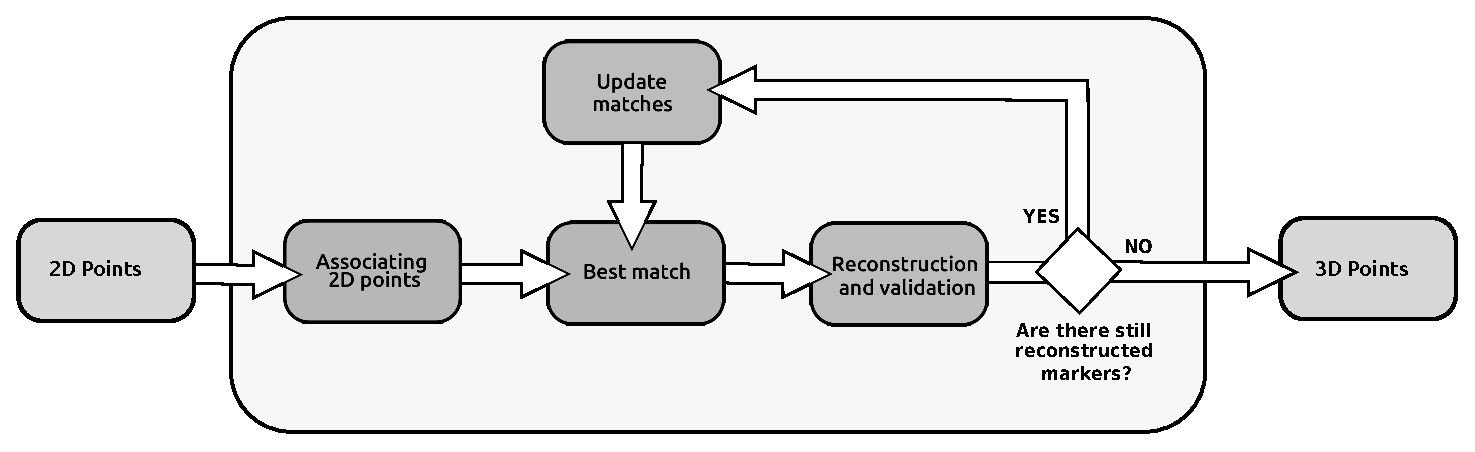
\includegraphics[scale=0.45]{./imagenes/Reconstruccion/bloques_reconstruccion}
        \caption{Diagrama de bloques del algoritmo de reconstrucción.}
        \label{fig: diagrama algoritmo}
    \end{center}
\end{figure}
%\vspace{-0.6cm}

\textit{Asociar puntos 2D}\label{seccion_asociar2D_uno}
%
Este bloque recibe como entrada las coordenadas de los puntos detectados en cada una de las cámaras, parámetros de las mismas tales como sus matrices de proyección y devuelve para cada punto una lista ordenada por relevancia, de las asociaciones existentes con puntos en otras cámaras.\\ 
%Los pasos a seguir son los siguientes:
%Basándose en lo explicado anteriormente para un par de cámaras el proceso  se puede ejemplificar  en la Figura \ref{fig: cam2cam } y los pasos a seguir son los siguientes:
%\begin{figure}[ht!]
%\begin{center}
%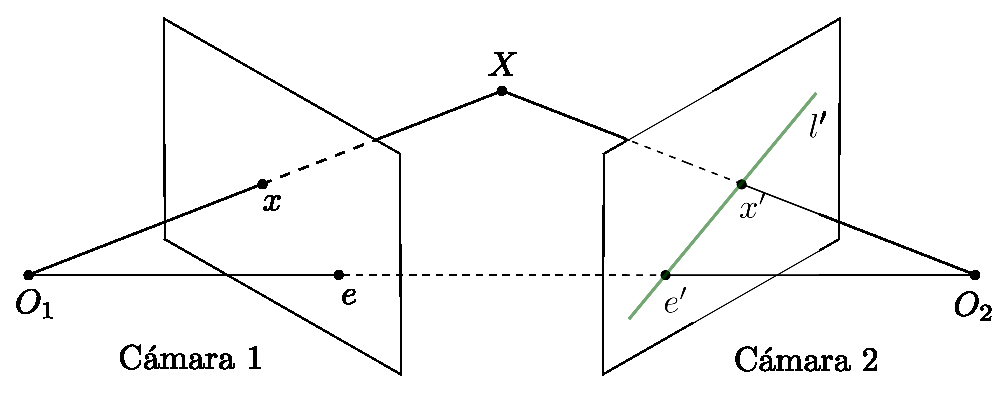
\includegraphics[scale=0.4]{/imagenes/Reconstruccion/geometria_epipolar}
%\caption{Asociación de puntos 2D en dos cámaras.}
%\label{fig: cam2cam }
%\end{center}
%\end{figure}
%\begin{itemize}
%\item Seleccionar dos cámaras y considerar un punto en una de ellas, por ejemplo el punto $x_{11}$ de la cámara 1.
%\item Proyectar la recta epipolar $l_{11}$ correspondiente al punto $x_{11}$ sobre la cámara 2.
%\item Tomar las distancias de los puntos detectados en la cámara 2 a la recta $l_{11}$.
%\item Generar una lista de posibles asociaciones ordenada por distancia.
%\end{itemize}
%Se asume que los puntos de la cámara 2 que tengan mayor posibilidad de corresponder con el punto $x_{11}$, son los más próximos a $l_{11}$.
%Repitiendo el procedimiento de manera inversa, esto es, de la cámara 2 a la cámara 1, se obtiene igualmente para cada punto de la cámara 2  los puntos de la cámara 1 ordenados según su proximidad a la recta epipolar correspondiente. A continuación se toman otros pares de cámaras y se vuelve a repetir el proceso. 
\textit{\hspace*{0.5cm}Mejor asociación.}\label{MejorAsociacion}
%
A partir de la lista con asociaciones entre pares de cámaras es necesario elegir aquella que posea mayor probabilidad de conformar la pareja de imágenes correspondiente a la proyección de un marcador 3D sobre dichas vistas.
%
Sobre cada par de cámaras se toma aquella asociación que posea la menor distancia y contenga puntos válidos, descartando las restantes. % Un punto se considera válido si en iteraciones anteriores no se a podido asociar a ningún punto 3D reconstruido.
%De esta forma cada punto de una cámara es asociado, si existen puntos válidos, con un punto en otra de las cámaras.
%
%Para evaluar de todas las relaciones entre cámaras, cuál de los pares de puntos asociados disponibles es el par que posee mayor posibilidad de corresponder a las proyecciones de un punto 3D, se proyectan los rayos de proyección de todos los pares de puntos disponibles y se toma el par que genere rayos de proyección con la menor distancia entre sí.
%\begin{tabbing}
%xx\=xx\=xx\=xx\=xxxxxxxxxxxxxxxxxxxxxxxxxxxxx\=xx\=x\kill
%\textbf{Algoritmo:} \textit{Asociar puntos 2D.}                       \>\>\>\>\>\textbf{Algoritmo:} \textit{Mejor asociación.}\\
%$\forall$ cámara $i$ y $j\not=i$                 \>\>\>\>\> $\forall$ cámara $i$ y $j\not=i$\\
%\>$\forall$ punto $x_{in}$ en cámara $i$              \>\>\>\>\>$\tilde{D}_{ij}=$ válidos$(D_{ij})$\\
%\>\>Hallar recta epipolar $l_{in}$ en cámara $j$     \>\>\>\>$b_{nm}^{ij}=$ mínimo$(\tilde{D}_{ij})$\\
%\>\>$\forall$ punto $x_{jm}$ en cámara $j$              \>\>\> \>$x_{in} x_{jm}$ pareja asociada a $b_{nm}^{ij}$\\
%\>\>\>$b_{nm}=$ distancia$(x_{jm}, l_{in})$                 \>\>\>$d_{ij}=$ distancia entre rayos de $x_{in}$ e $x_{jn}$\\
%\>\>$D_{ij}=\{b_{nm}\}$, posibles asociaciones       \>\>\> $d=$ mínimo$(\{d_{ij}\})$
%\end{tabbing}
\vspace{-0.65cm}
\begin{figure}
    \begin{center}
       \includegraphics[scale=1.0]{./imagenes/Reconstruccion/Algoritmo_reconstruccion}       
    \end{center}
\end{figure}
\vspace{-1.0cm}

Es importante resaltar que para la elección de los pares de cámaras se han considerado dos casos.
El primero de ellos evalúa cada cámara respecto a todas las restantes y el segundo considera la disposición de las cámaras en el espacio y empareja las cámaras adyacentes de manera consecutiva.

\textit{Reconstrucción 3D y validación.}\label{seccion_reconstruccion3D_validacion}
La pareja de puntos $x_i x_j$ de las cámaras $i$ y $j$ respectivamente, reconstruyen un punto 3D $X_{ij}$ válido si existe al menos un $x_k$ en cámara $k\not= i, \,j$ tal que $X_{ik} \in $ Bola$(X_{ij}, \delta)$, para cierto umbral $\delta$.
%
%Luego de encontrar la mejor asociación de puntos se procede a reconstruir y validar la misma. 
%Si se encuentra al menos un punto en otra cámara que valide la reconstrucción se asume que ésta es correcta, se retira a la pareja que genera la reconstrucción así como también a los puntos que lograron validarla y se itera nuevamente repitiendo el proceso con la siguiente mejor pareja asociada entre dos cámaras.  
%
%\begin{figure}[ht!]
%\begin{center}
%%\includegraphics[scale=0.4]{/imagenes/Reconstruccion/validacion}
%\caption{Reconstrucción entre cámaras 1, 2 y validación con cámara 3.}
%\label{img_reconstruccion_validacion}
%\end{center}
%\end{figure}
%
%La información que contiene un punto en una retina se mapea en el espacio 3D sobre el rayo de proyección que contiene a dicho punto y al centro de la cámara correspondiente. Supongamos que se tienen los rayos de proyección en el espacio 3D de todos los puntos contenidos en las retinas y que $x_1$ es un punto en la cámara 1 y $x_2$ es un punto en la cámara 2 que se encuentran asociados y reconstruyen al punto $X_{12}$. El algoritmo implementado asume que un punto en alguna cámara, valida a $X_{12}$ si junto a $x_1$ reconstruye un punto 3D que se encuentra dentro de la esfera $B(X_{12}, \delta)$ de centro $X_{12}$ y radio $\delta$, donde $\delta$ es un cierto valor umbral. %Como se muestra en la Figura \ref{img_reconstruccion_validacion}, el punto $x_3$ de la cámara 3 valida la reconstrucción, no así el punto $\tilde{x}_3$. 
%
%Idealmente $X_{12}$ se genera al interceptar los rayos de proyección de los puntos $x_1$ y $x_2$, pero debido a incertidumbres en la detección de marcadores o la calibración, comúnmente los rayos se van a cruzar. La reconstrucción, se estima como el punto del espacio de menor distancia a ambos rayos. %, por lo que $X_{12}$ se encuentra en el punto medio del segmento perpendicular a ambos rayos.

\textit{Actualizar asociaciones.}\label{actualizar_asociaciones}
%Del bloque anterior se tiene, un punto $X$ reconstruido y sus correspondientes proyecciones en cada una de las cámaras. Dichas proyecciones no deben ser consideradas nuevamente, por tanto estos puntos 2D que reconstruyen $X$, no se consideran como puntos válidos en las siguientes iteraciones.
%Los puntos 2D sobre las cámaras asociados a la reconstrucción del punto 3D $X$ no deben ser considerados nuevamente, por tanto estos puntos 2D se consideran como puntos no válidos en las siguientes iteraciones.
Se retira la pareja que genera la reconstrucción $X_{ij}$ así como también a los puntos $x_k$ que lograron validarla y se itera nuevamente repitiendo el proceso con la siguiente mejor pareja asociada entre dos cámaras.
%
%Finalmente el proceso iterativo se detiene cuando no hay más marcadores para reconstruir, lo cual implica que se cumple alguna de las siguientes condiciones:
%\vspace{-0.3cm}
%\begin{itemize}
%\item el número de marcadores reconstruidos es igual al número de marcadores que tiene colocada la persona, o igual al número máximo de marcadores  reconstruidos que se haya indicado.
%\item No existen puntos 2D válidos tal que pueda establecerse una asociación entre puntos de distintas vistas.
%\end{itemize}
Finalmente el proceso iterativo se detiene cuando el número de marcadores reconstruidos es igual al número de marcadores que tiene colocada la persona, igual al número máximo de marcadores reconstruidos que se haya indicado, o no existen puntos 2D válidos tal que pueda establecerse una asociación entre puntos de distintas vistas.